\def\thelstlisting{}

%不需要区分奇偶页的请使用下面一行
\documentclass[a4paper,AutoFakeBold,oneside,12pt]{book}
%需要区分奇偶页的(即每一章第一页一定在奇数页上)请使用下面一行
%\documentclass[a4paper,AutoFakeBold,openright,12pt]{book}
\usepackage{BUPTthesisbachelor}
\usepackage{setspace}

%\lstdefinestyle{sharpc}{language=[Sharp]C, frame=lrtb, rulecolor=\color{blue!80!black}}


%%%%%%%%%%%%%%%%%%%%%%%%% Begin Documents %%%%%%%%%%%%%%%%%%%%%%%%%%
\begin{document}

% 封面
\blankmatter
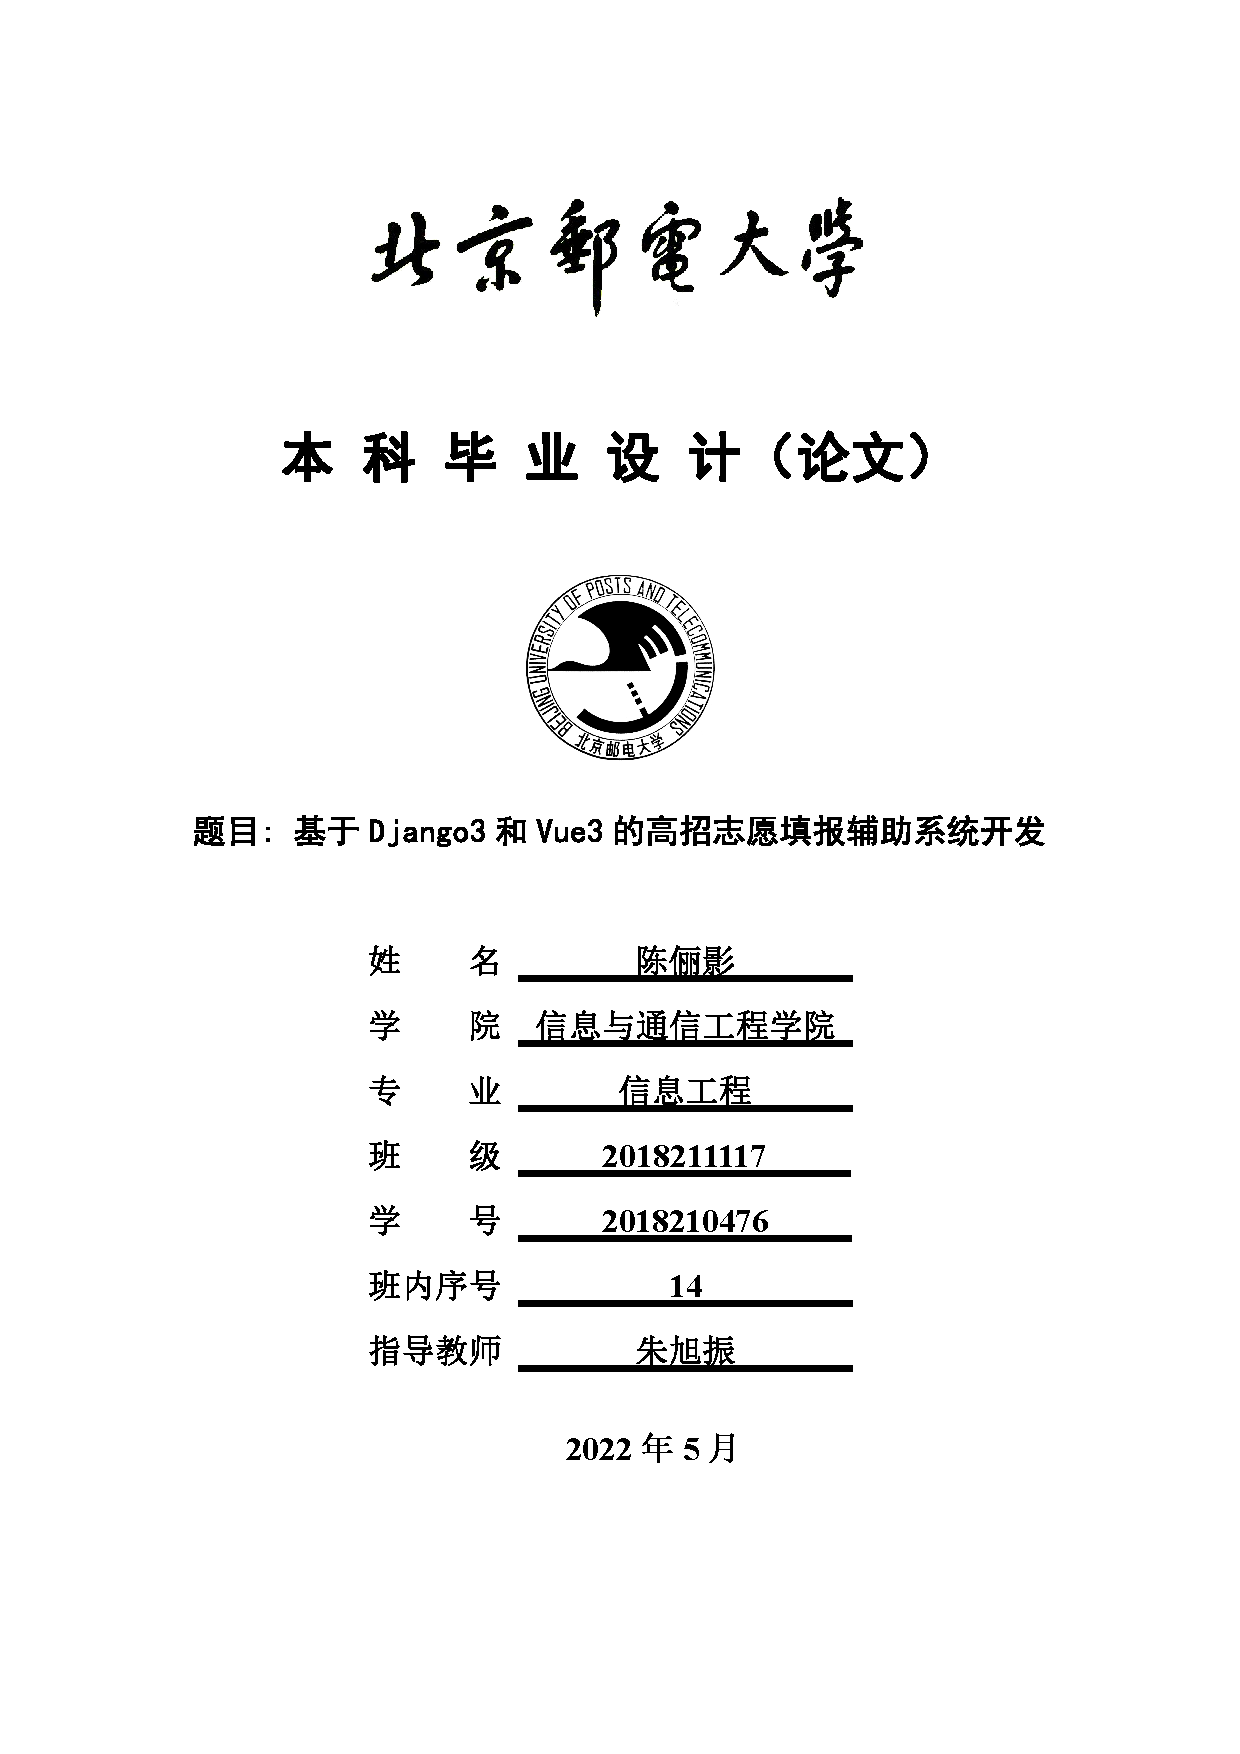
\includepdf[pages=-]{docs/cover.pdf}  

% 任务书
\blankmatter
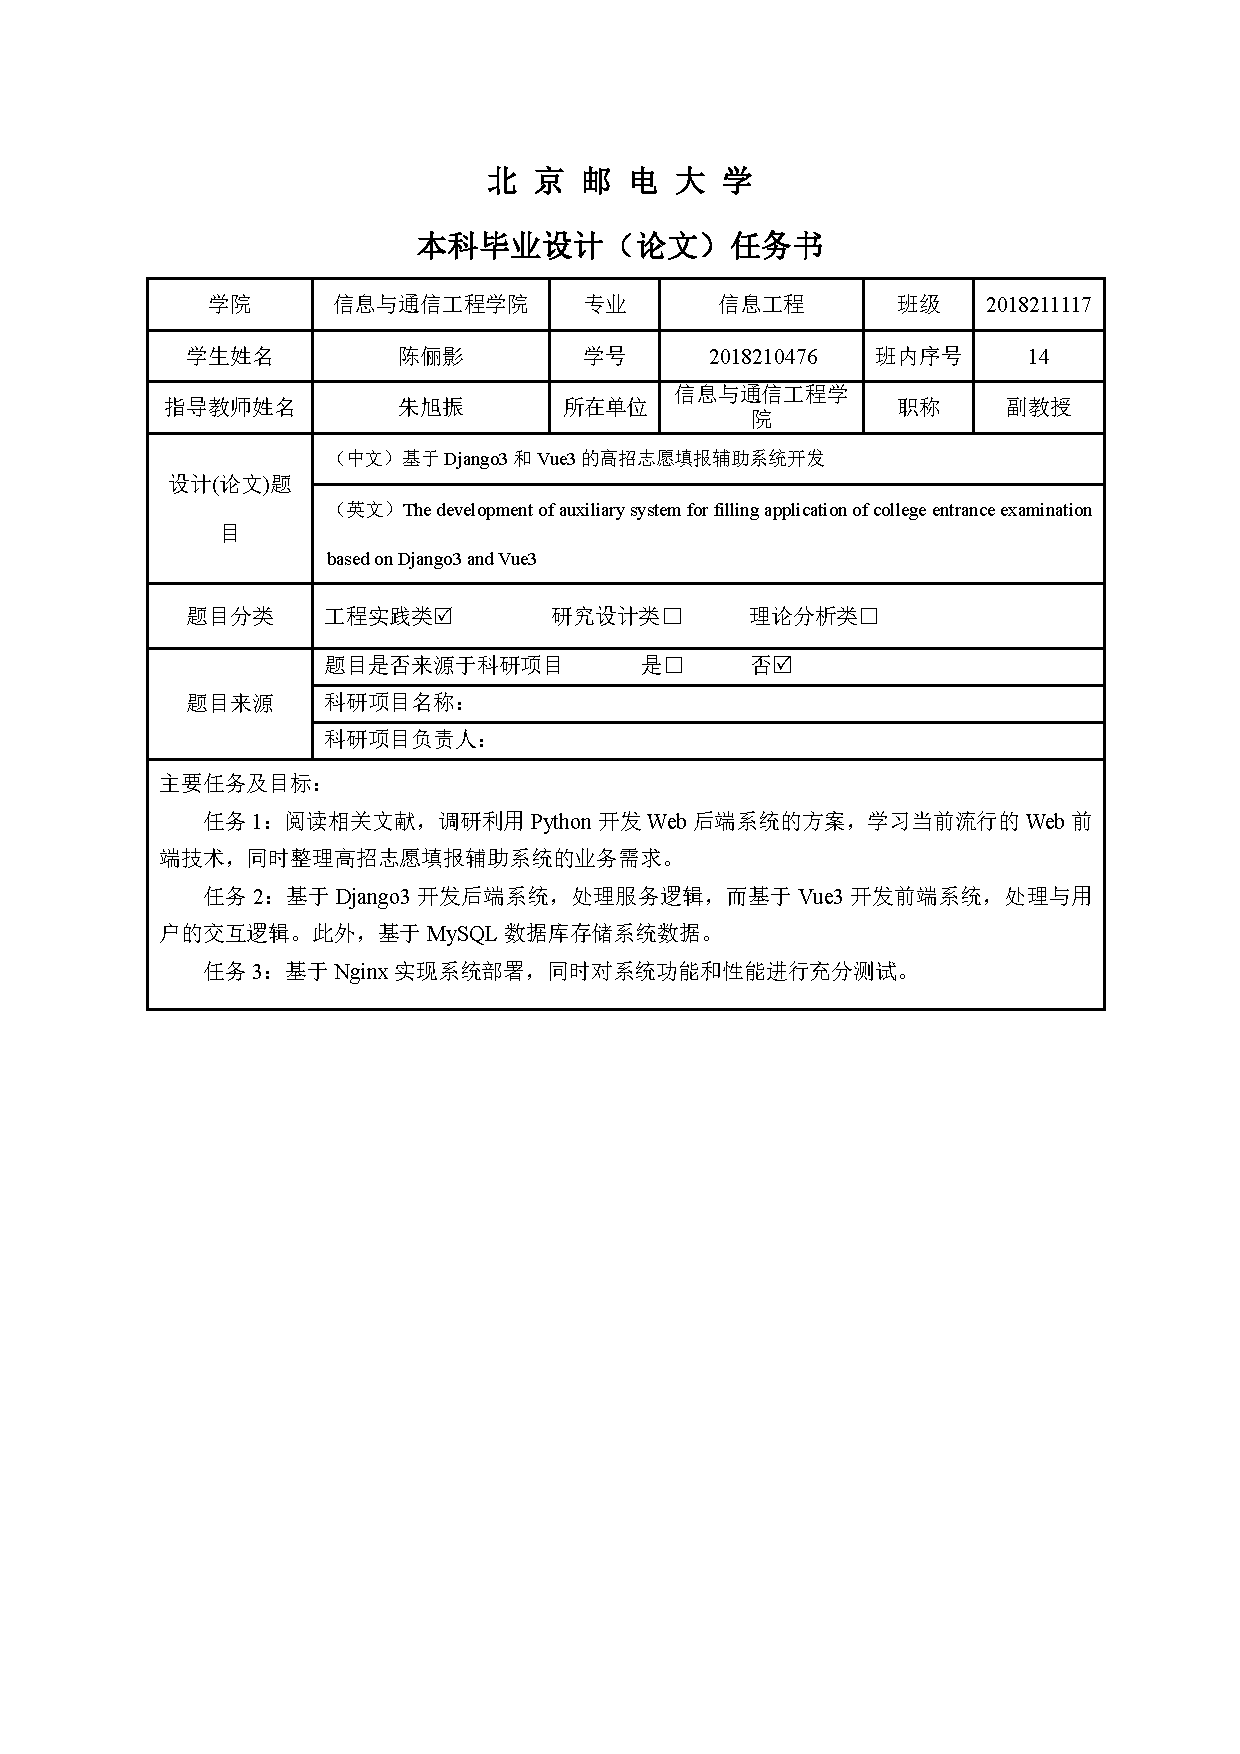
\includepdf[pages=-]{docs/task.pdf}  

% 成绩评定表
\blankmatter
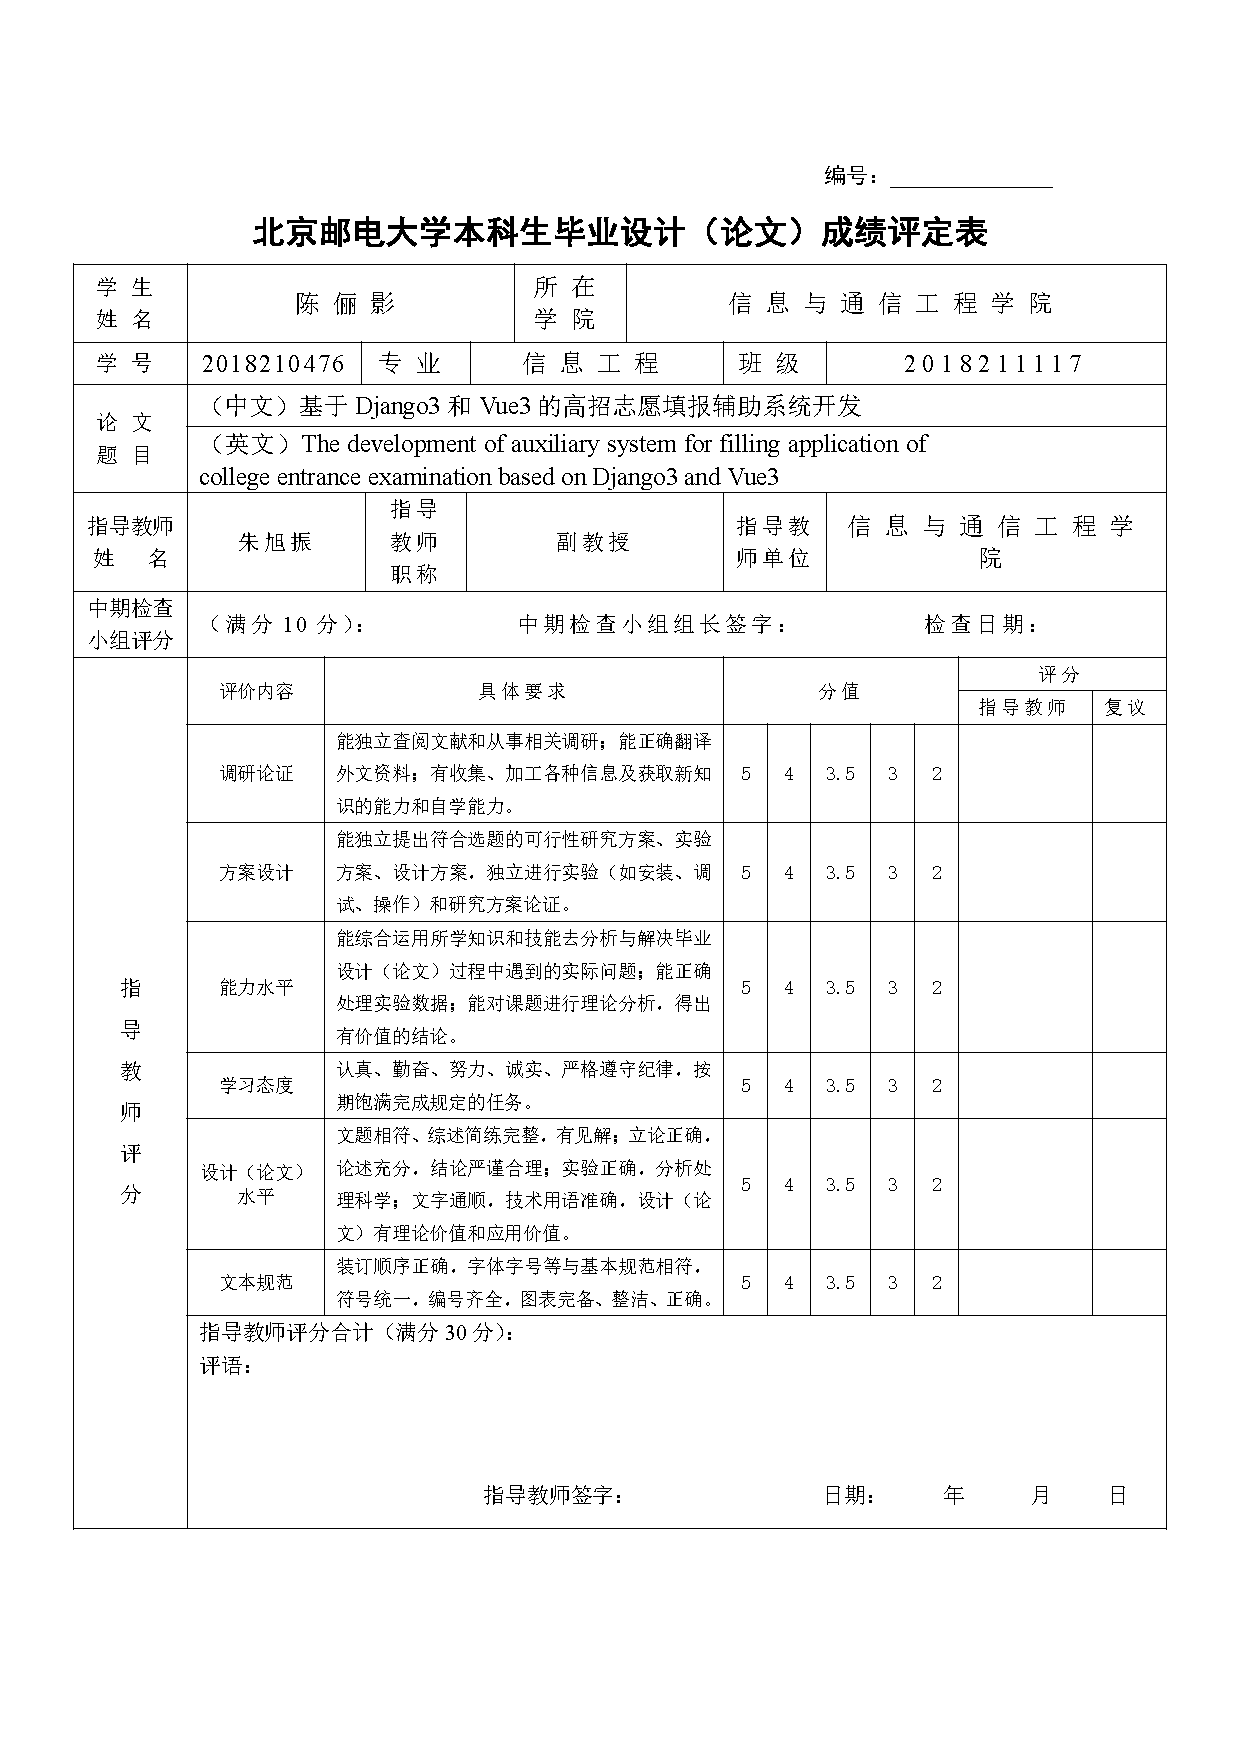
\includepdf[pages=-]{docs/scoreTable.pdf}  

% 诚信声明
\blankmatter

\includepdf[pages=-]{docs/statement.pdf} 

%%%%%%%%%%%%%%%%%%%%%%%%%%%%%%%%%%%%%%%%%%%%%%%%%%%%%%%%%%%%%%%%%%%%
%                                                                  %
%   Copyright (c) 2010 - 2011 Caspar Zhang <casparant@gmail.com>   %
%                                                                  %
%   This copyrighted material is made available to anyone wishing  %
%   to use, modify, copy, or redistribute it subject to the terms  %
%   and conditions of the GNU General Public License version 2.    %
%                                                                  %
%   This program is distributed in the hope that it will be        %
%   useful, but WITHOUT ANY WARRANTY; without even the implied     %
%   warranty of MERCHANTABILITY or FITNESS FOR A PARTICULAR        %
%   PURPOSE. See the GNU General Public License for more details.  %
%                                                                  %
%   You should have received a copy of the GNU General Public      %
%   License along with this program; if not, write to the Free     %
%   Software Foundation, Inc., 51 Franklin Street, Fifth Floor,    %
%   Boston, MA 02110-1301, USA.                                    %
%                                                                  %
%%%%%%%%%%%%%%%%%%%%%%%%%%%%%%%%%%%%%%%%%%%%%%%%%%%%%%%%%%%%%%%%%%%%

% 你只需要修改下面几行就可以完成大部分内容的填写,
% 这要求你具有一定的LaTeX基础,但是如果你足够聪明,
% 不具有LaTeX基础也可以完成。

% 论文中文题目
\def\thesistitle{基于Django3和Vue3的高招志愿填报辅助系统开发}

% 论文英文题目
%提示:英文摘要页的标题注意格式要求。
\def\thesistitleen{The development of auxiliary system for filling application of college entrance examination based on Django3 and Vue3}

% Thank Words
\def\thankwords{

此处请写致谢的内容。

它可以有多段。
}
    % Main items 
%%%%%%%%%%%%%%%%%%%%%%%%%%%%%%%%%%%%%%%%%%%%%%%%%%%%%%%%%%%%%%%%%%%%
%                                                                  %
%   Copyright (c) 2010 - 2011 Caspar Zhang <casparant@gmail.com>   %
%                                                                  %
%   This copyrighted material is made available to anyone wishing  %
%   to use, modify, copy, or redistribute it subject to the terms  %
%   and conditions of the GNU General Public License version 2.    %
%                                                                  %
%   This program is distributed in the hope that it will be        %
%   useful, but WITHOUT ANY WARRANTY; without even the implied     %
%   warranty of MERCHANTABILITY or FITNESS FOR A PARTICULAR        %
%   PURPOSE. See the GNU General Public License for more details.  %
%                                                                  %
%   You should have received a copy of the GNU General Public      %
%   License along with this program; if not, write to the Free     %
%   Software Foundation, Inc., 51 Franklin Street, Fifth Floor,    %
%   Boston, MA 02110-1301, USA.                                    %
%                                                                  %
%%%%%%%%%%%%%%%%%%%%%%%%%%%%%%%%%%%%%%%%%%%%%%%%%%%%%%%%%%%%%%%%%%%%

% 你只需要修改下面内容就可以完成中英文摘要,
% 这要求你具有一定的LaTeX基础,但是还是那句话,
% 如果你足够聪明,不具有LaTeX基础也可以完成。

% 中文摘要
\def\abstractzh{
%从这里开始写你的摘要,分段需要空一行。
高考志愿填报是中国的每位高中生不可忽视的人生重要选择,而对于许多学生,尤其是来自经济和教育水平不高的地区的学生,他们将大部分的精力都放在如何考好试上,而对于志愿填报不甚了解。如果没有得到好的指导,一位学生可能会因为信息不对称而在志愿填报上吃亏,没有进入一个符合自己分数的学校,甚至被退档以至无学可上,这会是一个很大的遗憾。因此,在高考结束后,帮助学生完成一个好的志愿选择是一项普惠性的、符合应试教育国情的工作。本毕业设计将致力于开发一个能够充分照顾学生的需求、推荐算法合理、信息全面而准确、精简无累赘而又易于使用的高招志愿填报辅助系统,建设一个能够为广大考生和家长分忧的设施。

本志愿填报辅助网站的开发过程使用了前后端分离的形式,采用Django3.2作为框架、Python语言作为编程语言、PyCharm2021.3作为编辑器进行后端的开发,采用Vue3作为框架、HTML, CSS, Javascript语言作为编程语言、Visual Studio Code作为编辑器进行前端开发,使用MySQL数据库进行数据的管理,并使用Nginx进行反向代理搭建。网站的结构分为用户界面和管理员界面两个部分。管理员可以对用户、文章、院校资料等数据进行浏览及更改,而用户可以浏览院校资料库并进行定向查询、根据自己的成绩进行录取可能性的分析、模拟志愿填报,以及浏览各类新闻信息等。

本文将详细地对该网站的开发过程以及实现的功能进行介绍,包括整体构思、开发环境、各大模块的功能及开发过程等。
%摘要结束
}

% 中文关键字 
% TODO: 改成可变长度的
\def\abszhkeyone{Vue}
\def\abszhkeytwo{Django}
\def\abszhkeythree{MySQL}
\def\abszhkeyfour{线性回归}
\def\abszhkeyfive{高考志愿}

% ABSTRACT
\def\abstracten{
%Your abstract here, to make a new paragraph, give an extra blank line please.
The college entrance examination is an important choice in the life of every high school student in China that cannot be ignored, and for many students, especially those from areas with low economic and educational levels, they focus most of their energy on how to do well on the exams and do not know much about filling applications. Without good guidance, a student may lose out on applications due to information asymmetry, not getting into a school that matches his or her score, or even being dropped or even having no school to go to, which can be a big regret. Therefore, helping students to complete a good application selection after the college entrance examination is a universal and in line with the national situation of test-based education. This graduation design will be devoted to developing a high school entrance examination application assistance system that can fully take care of students' needs, a reasonable recommendation algorithm, comprehensive and accurate information, streamlined and non-cumbersome but easy to use, and building a facility that can share the worries of the majority of candidates and parents.

The development process of this volunteer application assistance website uses the form of front-end and back-end separation, using Django3.2 as the framework, Python language as the programming language, PyCharm2021.3 as the editor for the back-end development, using Vue3 as the framework, HTML, CSS, Javascript language as the programming language, Visual Studio Code as the editor for front-end development, MySQL database for data management, and Nginx for reverse proxy construction. The structure of the website is divided into two parts: user interface and administrator interface. The administrator can browse and change data such as users, articles, and college information, while users can browse the college database and make targeted inquiries, analyze the possibility of admission based on their scores, simulate filling applications, and browse various news and information.

In this paper, we will introduce the development process of the website and its functions in detail, including the overall concept, development environment, functions of major modules and development process.
%Abstract done
}

% Key Words 
% TODO: 改成可变长度的
\def\absenkeyone{Vue}
\def\absenkeytwo{Django}
\def\absenkeythree{MySQL}
\def\absenkeyfour{Linear Regression}
\def\absenkeyfive{University Application}


  % Abstract
\fancypagestyle{plain}{\pagestyle{frontmatter}}
\frontmatter\tableofcontents % Content


% 正文
\newpage\mainmatter
\fancypagestyle{plain}{\pagestyle{mainmatter}}
%\let\cleardoublepagebak=\cleardoublepage
%\let\cleardoublepage\relax % Make new chapter stay on old page

%%%%%%%%%%%%%%%%%%%%%%%%%%%%% Main Area %%%%%%%%%%%%%%%%%%%%%%%%%%%%

\chapter{绪论}

\section{研究背景及意义}
高考志愿填报一直以来是所有高中学生及家长的重要挑战。在经历了高考的苦战过后,许多学生和家长可能忽视或是没有能力去获取足够的信息来完成一个合适的志愿选择。尤其是来自经济和教育水平不高的地区的学生,更可能因为信息不对称而在志愿填报上面吃亏,没有进入一个整体情况适合自己且符合自己分数的学校,或者不能够选择一个适合自己的专业。想要顺利地填报志愿,需要获取充沛的信息和进行恰当的分析,而一个好的平台能够集中这些资源,从而帮助许多需要的学生找到自己梦想的起跳板。

目前我国各高考地区采用的志愿填报方式仍处于新旧模式并存的状态,其中对于填报的时间分为“考前填报”(旧式,在部分地区依然沿用)和“知分填报”(新式,大多数地区采用),而志愿录取模式则分为“顺序志愿”(旧式)和“平行志愿”(新式)。目前来说,大部分地区都采取了知分填报和平行志愿的模式,因此本设计可能会更偏向于这些模式,但其中的主要功能(根据分数来考虑学校的录取可能性以及各类信息检索等)依然是对这几种模式下的志愿填报都有所助益的。直至今年,部分地区依然使用文理分科法,而部分地区已经采取"3+3"或"3+1+2"等新高考的模式。\cite{我国高考志愿填报机制的演变与优化}如何做到对于新高考改革的适应也是在开发高考志愿填报辅助系统的过程中一项十分重要的工作。

因此,开发一个能够充分照顾学生的需求、推荐算法合理、信息全面而准确、精简无累赘而又易于使用的高招志愿填报辅助系统是一件非常有意义的事情。本毕业设计将集中完成这样的一个目标,建设一个能够为广大考生和家长分忧的设施。

\section{国内外有关本选题研究的动态}
国外的大学升学模式与国内普遍存在明显差别,一般采用单独向学校申请的方式,录取的影响因素也较多。而我国高考升学的志愿填报方式较为简单,以分数为唯一参照,因此本毕业设计的研究过程也主要考察国内的高考志愿填报方式,以及国内的相关产品及研究。

在市面上已经出现一些指导高考志愿填报的系统,如教育部的官方平台“阳光高考”、“掌上高考”、“完美志愿”等。但它们中许多设计不够完善,没有办法根据学生的成绩以及不同学生的需求(专业偏向、城市偏向、学校类型或规模偏向)来指导学生进行填报志愿的选择;有一些系统的推荐算法只根据往年分数,而不考虑试题的难度,容易造成较大的误差;有一些系统的信息获取不够全面,挖掘得不够深入,可能无法提供准确的分析;有一些商业化系统则过于重视营收,没有做好帮助学生选择学校和专业的本职,而是把重心放在了没有必要的内容上;还有一些由于技术有限等原因,客户端界面不够人性化、不易于使用。

在本毕业设计的研究过程中,对这些相关产品的相关功能进行了分析,在确定本毕业设计的功能的过程中有一定的参考,并力图规避它们的不足之处。


\section{论文的结构}




\chapter{相关开发技术}

\section{Python 网络爬虫}
在本毕业设计的开发过程中,需要使用大量的真实高考录取数据和院校资料来进行功能的试验以及页面内容的填充,因此在本毕业设计中主要使用 Python 网络爬虫这一高效率的方式获取数据。

\subsection{Python 语言}
Python 是一种广泛使用的解释型、高级和通用的编程语言。Python 支持多种编程范型,包括函数式、指令式、反射式、结构化和面向对象编程。它拥有动态类型系统和垃圾回收功能,能够自动管理内存使用,并且其本身拥有一个巨大而广泛的标准库。\cite{python_wikipedia}\cite{python_about}

在本毕业设计中大量使用 Python 语言来进行一些爬虫及数据处理脚本的编写,其优势在于学习成本较低,并且拥有易于使用、安全规范的外部包管理系统和活跃的社区生态。活跃的社区生态使得许多公开发布的有用功能可以直接被应用到程序中,开发者无需闭门造车,对于较大规模程序的开发,使用 Python 语言引入相关库能达到事半功倍的效果。

目前仍在广泛使用的 Python 语言版本分别为 Python 2 和 Python 3, 本毕业设计中均使用 Python 3 环境进行开发。

\subsection{网络爬虫}
网络爬虫是一种互联网机器人,它通过特定的模式在互联网上进行索引,浏览海量的网页,并从 HTML(超文本标记语言,HyperText Markup Language)代码中提取信息进行下载。\cite{web_crawler}

本毕业设计中,网络爬虫的部分使用 Python 语言进行编写,这也是目前主流的网络爬虫编写方式。本设计中的爬虫主要使用的 Python 库有 urllib(url 处理模块,Python 标准库之一,用来处理 url 请求)\cite{urllib}以及 lxml(Python 平台的 XML 和 HTML 工具包,用来进行 XML 或 HTML 解析,提取需要的内容)\cite{lxml}. 

\section{Django 后端}
Django 是一个免费、开源的高级 Python Web 框架,具有比较完善的功能,并且有着较高的安全性,通常来说是使用 Python 语言进行 Web 开发的一个主要的选择。Django 采用了 MVT 的软件设计模式:视图、模型和模板。\cite{django}\cite{django_runoob}Django 的模型系统相对于传统的直接操作数据库的方式功能性更强,并且能同步注册到后台管理界面,在本毕业设计中发挥了显著的作用。

本毕业设计中采用 Django 3.2 版本进行后端开发,其中负责的程序包括用户认证系统、数据模型的管理以及 API(应用程序接口,application programming interface)的开放,并且管理员端的界面采用的也是Django的原生后台管理系统。

\section{Vue 前端}
本毕业设计中,前端部分使用 HTML, CSS, JavaScript 语言,配合 Vue 框架完成页面显示的实现。

\subsection{Web 前端开发编程语言}
Web 前端开发的核心构成通常为以下三种开发语言:HTML, CSS, JavaScript. 它们在生成网页的过程中分别产生不同的作用。

\begin{itemize}
\item \textbf{超文本标记语言}(Hypertext Markup Language,简称:HTML)是一种用来结构化 Web 网页及其内容的标记语言,相当于建筑的框架。在 Web 网页的构成中,它是最为基本且无法缺少的部分。\cite{html_mdn}

\item \textbf{层叠样式表}(Cascading Style Sheet,简称:CSS)是为网页添加样式的代码,相当于建筑的装修粉饰。样式表可以为网页增加适当的排列、色彩等样式,实现美观性。\cite{css_mdn}

\item \textbf{JavaScript} 是一门编程语言,可为网站添加各种交互功能。标准化的 JavaScript 被称为 ECMAScript(简称:ES),随着时代的更替,ES 的代码规范和语言性能也得到了修订和改进。\cite{javascript_mdn}实际使用时,大型项目很少完全使用原生 JavaScript 进行编程,很多时候会配合 React, Vue, Angular 等框架来实现更强大的功能和规范化。
\end{itemize}

\subsection{Vue 框架}
Vue.js 是一款用于构建用户界面的渐进式 JavaScript 框架,是目前非常主流的 JavaScript 框架之一。Vue 框架的设计理念是自底向上的。它的核心库只关注视图层,不仅易于上手,还便于与第三方库或既有项目整合。对于复杂的单页应用,使用 Vue 框架是非常有优势的。\cite{vuejs}

目前广泛使用的 Vue 框架有 Vue 2 和 Vue 3 两种版本,本毕业设计采用的是更新版的 Vue 3. 新的版本解决了旧版本的一些问题,还能使工程更加体系化。

\subsection{Vite}
Vite 是构建 Vue 3 工程的一款开箱即用的脚手架。它能够快速地构建一套 Vue 生产环境,能够安装一些插件,并且有一个支持热更新(即更新代码后实时将更新反馈到页面)的开发服务器。\cite{Vite}

本毕业设计采用 Vite 构建 Vue 3 框架的前端工程,并使用配套的开发服务器进行一系列的系统功能测试。

\section{Web 前后端分离}
Web 前后端分离式开发是近年来 Web 开发的热门模式,通过将前后端的开发流程进行解耦,达到一个双管齐下、互不干扰的效果,能够提高工程师的工作效率和代码的可维护性。下文将会介绍 Web 前后端分离式开发的一些流程以及使用的工具。

\subsection{前后端分离式开发流程}
前后端分离的工作流程主要如下:前后端工程师确定产品功能,以及接口和传递的数据类型;前端工程师以空数据或虚拟数据的状态开发前端界面,同时后端工程师设计后台计算逻辑并暴露接口;这些开发完成后,前端工程师就可以通过 Ajax 等方式访问接口调取数据,从而实现一个完整的程序。

\subsection{Vue Router}
传统的 Web 开发模式下,浏览器访问的页面往往是服务器直接返回的整个 HTML 文件,而前后端分离式开发则把页面跳转的工作交给前端实现,也就是现在所说的前端路由。这种模式下,对网页 HTML 结构以及静态资源的请求是不会受后端服务器状态的影响的。

Vue Router 是 Vue.js 的官方路由。在使用 Vue 框架开发单页应用时,一般使用它来负责前端路由,它会接管浏览器的操作(如刷新、后退)来使得前端路由的体验接近用户的预期。\cite{vue_router}本毕业设计中使用 Vite 的插件管理模块安装 Vue Router 并实现前端路由。

\subsection{Axios}
Axios 是一个基于 promise(JavaScript 中一种常用的异步方式)的 HTTP 请求工具。\cite{axios}它是一种 Vue 框架开发者主流的调取 API 的方式。本毕业设计中也使用 Vite 的插件管理模块安装 Axios 以实现前后端 API 通信。

\section{MySQL}
MySQL 是 Oracle 公司开发的一款基于 SQL 语言的关系型数据库。它是比较传统的一款关系型数据库,具有扎实的功能和稳定性。\cite{mysql}本毕业设计使用开源版的 MySQL 作为数据库,它与 Django 有着良好的兼容性。在数据处理的过程中也常使用 pymysql 库在 Python 脚本中对 MySQL 数据库进行读写操作。

\section{Nginx}
Nginx 是一个异步框架的网页服务器,通常也可以用作反向代理、负载平衡器和 HTTP 缓存。\cite{nginx}本毕业设计中使用 Nginx 将前后端的开发服务器代理到同一域名下,解决同源策略问题,实现一个整体的测试运行服务器。


\chapter{系统可行性分析}
在软件开发之前,对其进行可行性分析,分析其技术、经济、环境等方面的实践可行性,能够保证工程的实现是切合实际且具有以人为本的精神的。除此之外,对各方面的社会效益有一定的思考,能使得开发者在开发过程中更具备社会责任感。本章将从四个方面进行系统的可行性分析。

\section{技术可行性分析}
系统使用的是前后端分离的开发方式,使用的语言有 Python, HTML, CSS, JavaScript, 并使用 Vue 和 Django 框架,数据库使用 MySQL. 以上所运用的技术都是当前比较成熟的,安全性和可靠性都有着保障。并且这些技术运用得十分广泛,因此可以容易地得到系统的学习资料和问题参考。

\section{经济可行性分析}
高考一直是大部分中国学生的关键人生节点,在其无与伦比的重要性下,高考以及志愿填报的辅导具有着经久不衰的经济效益。这种类型的程序并不缺乏用户,维护强度不高,且使用率呈现一定的周期性,只要合理规划服务器的负载利用率,经济效益应当是合适的。

\section{操作可行性分析}
本程序是一款 Web 平台应用,在任何能运行网页浏览器的设备上均可运行,功能和页面交互也比较简单直观,对于能正常使用浏览器浏览网页的人几乎不需要学习成本。

\section{社会效益可行性分析}
本毕业设计的选题意在帮助广大的高中学生及家长更好地完成高考志愿的选择。对于经济实力以及搜集信息能力较弱的家庭,这样的系统可能会有很大的帮助,因此本毕业设计会基于这样的普惠性的想法来完成。


\chapter{系统构思设计}
在启动正式的开发进程之前,一个精密的整体构思是不可或缺的。有了良好的构思,可以预见并提前避免做一些无用功,并使开发者对任务的完成进度有更好的掌握。本章将分别介绍功能模块、应用内部模块以及数据库的设计。

\section{功能模块设计}
客户端功能模块整体的思路设计图见图\ref{function_modules}, 包括了填报指导、高校信息、新闻政策、用户系统四个模块。此外,管理后台将作为一个单独的模块进行介绍。
\buptfigure[width=1\textwidth]{pictures/客户端功能模块设计图}{客户端功能模块设计图}{function_modules}

\subsection{填报指导模块设计}
填报指导模块又分为以下几个子模块:院校资料库、录取可能性分析、模拟志愿填报、一分一段表。
\subsubsection{院校资料库}
本模块主要是为用户提供浏览数据库各类大学资料的功能。院校资料库模块在本系统中具有一定的重要性,学生和家长可以根据自己的个性化需求去查询得到指定的院校信息,
\begin{itemize}
\item \textbf{院校列表:}通过院校名片的形式展示院校的名称、所在城市以及一些其他情况(办学性质、荣誉等)。并且用户可以通过所在省份、开设专业、办学性质、荣誉等方面进行筛选查看,也可以直接对院校名称进行搜索。
\item \textbf{院校详情:}点击院校名片会进入单独的页面,该页面展示了院校的名称、所在城市、简介、开设专业及往年录取分数等信息。其中,可以浏览不同报考地区的录取分数,但系统会自动读取用户的报考地区并优先显示。
\end{itemize}

\subsubsection{录取可能性分析}
本模块将会根据用户的个人资料中的成绩情况和期望报考的学校进行分析,然后显示用户录取的可能性。具体事件流程如图\ref{application_analyse}, 用户选择自己想要查询的学校后点击查询按钮,系统会在后台进行对该学校录取分数线或名次的预测,再读取用户资料中的成绩信息,将两者进行一个分析比对,并展示分析结果。
\buptfigure[width=1\textwidth]{pictures/录取可能性分析}{录取可能性分析流程图}{application_analyse}

\subsubsection{模拟志愿填报}
本模块的功能是为用户提供一个模拟填报的系统,让用户预先体验志愿填报的流程,并且根据不同的志愿顺序,结合用户的个人成绩进行院校的推荐。在选择院校填报的过程中,用户除了可以选择系统推荐的院校,也可以直接搜索自己选定的院校来进行填报。用户使用事件流程如图\ref{application_simulation}所示。
\buptfigure[width=1\textwidth]{pictures/模拟志愿填报}{模拟志愿填报流程图}{application_simulation}

\subsubsection{一分一段表}
本模块的功能是提供官方的一分一段表文件以供用户进行查阅比对。因为官方的一分一段表参考标准比较复杂,计划采用文章的形式直接呈现原始内容,而用户可以使用搜索的方式找到自己需要的内容。

\subsection{高校信息模块设计}
本模块的主要内容是展示国内各大高校的荣誉、评价等信息,以便学生和家长在选择院校方面进行一定的参考。为保证信息的客观性,本模块全部使用文章的形式呈现,展示原始的信息内容。

\begin{itemize}
\item \textbf{双一流评级:}收录至今为止的双一流评级信息,包括一流大学的评选以及一流学科建设院校列表。
\item \textbf{全国第四轮学科评估:}收录全国第四轮学科评估中各个学科的大学评级信息。
\item \textbf{高校综合排名:}收录各大有影响力的机构对于国内高校的综合排名情况。
\item \textbf{高校专业排名:}收录各大有影响力的机构对于国内高校的各专业排名情况。
\end{itemize}

\subsection{新闻政策模块设计}
本模块的主要内容是展示最新的有关高考、高考招生以及志愿填报的新闻政策,以便学生和家长及时接收到最新的资讯。为保证信息的客观性,本模块也全部使用文章的形式呈现,展示原始的信息内容。

\begin{itemize}
\item \textbf{高考最新政策:}收录官方渠道发布的各地区高考最新政策资讯。
\item \textbf{志愿填报最新政策:}收录官方渠道发布的各地区高考志愿填报最新政策资讯。
\item \textbf{院校招生最新政策:}收录各院校发布的该校招生最新政策资讯。
\end{itemize}

\subsection{用户管理模块设计}
本模块负责对学生或家长的用户账户进行管理,提供注册、登录、修改资料和密码的功能。用户管理模块也是本系统比较重要的功能,许多其他模块都依赖用户资料来个性化地提供服务或进行数据分析。

\subsubsection{用户注册}
用户注册模块要求用户输入用户名和密码以进行注册,并有一定的格式及安全性检测。在注册时要求用户输入高考相关资料(报考地区、成绩等),以便于在其他功能中长期的使用。用户注册的事件流程见图\ref{sign_up}所示。在输入账户名和密码后进行一次前端合法性检验,不通过时会提示原因,通过后方可进入下一阶段输入高考信息。最后提交注册时先进行前端检验,再进行后端检验,不通过的时候提示原因,通过后提示注册成功,并转到个人资料页面以示意用户填写更多可选资料。其中,填写高考信息的阶段可随时回退到上一阶段。
\buptfigure[width=1\textwidth]{pictures/用户注册}{用户注册流程图}{sign_up}

\subsubsection{用户登录}
用户登录模块提供使用用户名和密码进行登录的功能,以便程序获取用户的信息来实现一些应用的功能。用户登录的事件流程见图\ref{sign_in}所示。用户输入用户名和密码,点击按钮发送登录请求后,系统后台判断登录是否成功,如不成功则提示用户重新输入登录信息,如成功则跳转至用户浏览器历史记录的上一个页面,以方便用户继续使用系统。
\buptfigure[width=1\textwidth]{pictures/用户登录}{用户登录流程图}{sign_in}

\subsubsection{更改资料}
更改资料模块为用户提供查看目前的个人资料以及更改资料的功能。进入页面后系统从后台读取目前的个人资料信息并展示,用户可以更改个人资料。更改完毕后用户可以提交更改,系统进行检验后返回资料更改是否成功的结果。用户也可以随时点击“取消更改”的按钮来放弃更改的内容,重新查看原本的资料。

\subsubsection{安全管理}
安全管理模块设定的基本功能是更改密码。用户需要输入旧密码,并两次输入新密码来更改密码。如果旧密码正确,且两次输入的新密码一致,即可成功更改密码,否则更改失败,系统向用户提示错误原因。

\subsection{管理后台模块设计}
管理后台模块主要的功能是为系统管理员提供一个管理用户以及其他数据库资料的可视化平台。在本系统中,主要需要管理的资源包括专业列表、院校信息、院校历年录取分数线信息,以及各类文章。管理员能够在管理后台中简单地实现增加、编辑和删除这些资源的操作。

\section{应用内部模块设计}
上一节中介绍了应用使用时的功能模块设计,本节则将介绍应用内部如何进行模块的划分以及每个模块所承担的功能。应用内部模块基本的内容及关系见图\ref{inner_modules}.
\buptfigure[width=0.7\textwidth]{pictures/应用内部模块设计图}{应用内部模块设计图}{inner_modules}

\subsection{核心模块}
主要负责“录取可能性分析”和“模拟志愿填报”功能,这两个功能是系统的核心技术成分。其中该模块的后端部分包括用到的一些分析和推荐算法,以及基础的返回 API. 前端部分则负责这两个部分的页面的实现。

\subsection{用户模块}
该模块的后端部分包括用户资料模型、用户认证系统(注册、登录、修改密码等 API)、以及一些用户资料读取和更改的 API. 前端部分则负责上文中用户管理模块所有功能的页面实现。

\subsection{院校模块}
该模块的后端部分包括院校、专业和录取分数线的模型,以及读取上述模型的各种信息的 API, 核心模块也会用到该模块的模型或方法。前端部分则负责院校列表以及院校详情的页面实现。

\subsection{文章模块}
该模块负责所有需要使用文章形式展现的部分。后端部分包括文章模型以及读取文章详细内容的 API. 前端部分则是文章列表以及文章详细内容的页面实现。

\section{数据库设计}
上一节中提到了应用内部模块的一些模型,本系统的数据管理主要是依托 Django 的模型系统配合 MySQL

\chapter{系统实现与测试}

\section{开发与运行环境}
\subsection{开发环境}
\subsection{运行及测试环境}

\section{数据的获取}
\section{各功能模块的实现}
\section{系统测试}


\chapter{总结}

\section{毕业设计总结}
\section{未来展望}
%%%%%%%%%%%%%%%%%%%%%%% Main Area ENDs Here %%%%%%%%%%%%%%%%%%%%%%%%
%\let\cleardoublepage=\cleardoublepagebak

\begin{nopagenumber}
% Reference
\clearpage\phantomsection\addcontentsline{toc}{chapter}{参考文献}
\bibliographystyle{buptbachelor}
\refbodyfont{\bibliography{ref}}

% Thanks to page
\clearpage
\chapter{致\qquad{}谢}
\normalsize\thankwords

% Appendix
\setcounter{figure}{0} 
\renewcommand{\thefigure}{~附-\arabic{figure}~}
\setcounter{equation}{0} 
\renewcommand{\theequation}{~附-\arabic{equation}~}
\setcounter{table}{0} 
\renewcommand{\thetable}{~附-\arabic{table}~}
\setcounter{lstlisting}{0} 
\makeatletter
  \renewcommand \thelstlisting
       {附-\@arabic\c@lstlisting}
\makeatother


\chapter*{附\qquad{}录}
\phantomsection\addcontentsline{toc}{chapter}{附\qquad{}录}

\phantomsection
\addcontentsline{toc}{section}{附录1\quad{}缩略语表}
\section*{附录1\quad{}缩略语表}



\clearpage
\phantomsection
\addcontentsline{toc}{section}{附录2\quad{}数学符号}
\section*{附录2\quad{}数学符号}



\end{nopagenumber}

% 开题报告
\blankmatter

\includepdf[pages=-]{docs/openingReport.pdf} 


% 中期检查表
\blankmatter
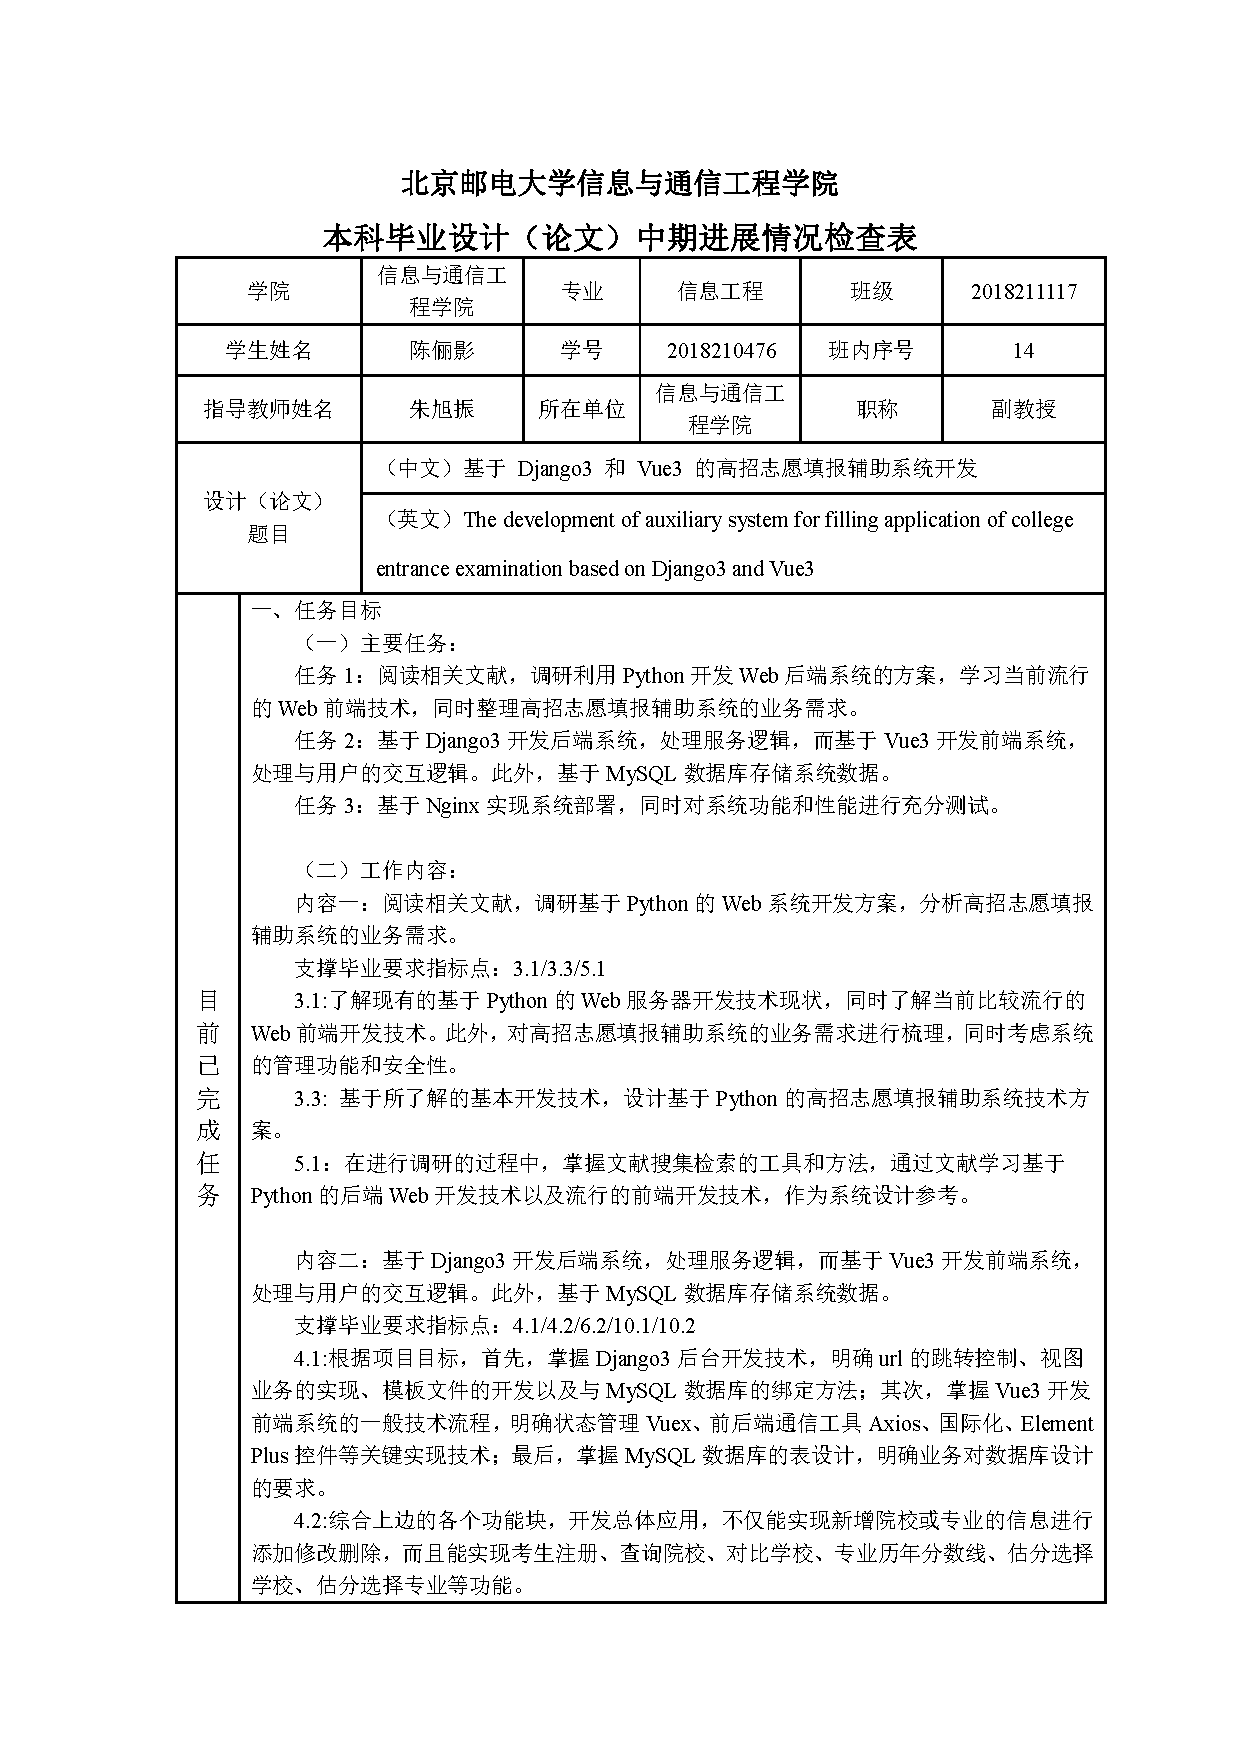
\includepdf[pages=-]{docs/interimReport.pdf} 


\end{document}
